\section*{Implementation of EKF}

An EKF was implemented according to the lecture slides. However, the gains are rather challenging to determine. 

However, the covariance matrices ($Q, R$), and the initial covariance matrix ($P_0$)
\begin{align*}
    Q &= \begin{pmatrix}
        0.05 & & \\ & 0.05 & \\ & & 0.05
    \end{pmatrix}, & 
    R &= \begin{pmatrix}
        0.08 & \\ & 0.2
    \end{pmatrix}, & 
    P_0 &= \begin{pmatrix}
        0.01 & & \\ & 0.1 & \\ & & 0.01
    \end{pmatrix},
\end{align*}

\fbox{\parbox{0.98\textwidth}{
    \textbf{How did I guess?}

    $Q$ is assumed as the variance in the model (not covariances, since it is a diagonal matrix) and since, in this case, $G$ (noise 'component' to the model), is non-existent, that is why low values of Q are assumed.

    $R$ is assumed as the variance in the measurement. High values are chosen because the gain is high. 

    $P_0$ is the initial co-variance matrix (how much we trust the initial guess), and low values are chosen for top-right and bottom-left since the initial guesses are quite good for $x$ and $\theta$, but the initial guess for $y$ is bad.
}}

A least-square optimization is performed to determine the matrices $Q$, $R$, and $P_0$. The matrices are
\begin{align*}
    Q &= \begin{pmatrix}
        8978 & & \\ & 0 & \\ & & 0.012
    \end{pmatrix}, & 
    R &= \begin{pmatrix}
        0 & \\ & 0.57
    \end{pmatrix}, & 
    P_0 &= \begin{pmatrix}
        1.33 & & \\ & 4.42 & \\ & & 0
    \end{pmatrix}
\end{align*}

The results of the optimization do not seem to agree with my guess. No idea why.

An array square-root algorithm was implemented and optimization resulted in the following covariance matrices:
\begin{align*}
    Q &= \begin{pmatrix}
        0.077 & & \\ & 0.0032 & \\ & & 0
    \end{pmatrix}, & 
    R &= \begin{pmatrix}
        1.511 & \\ & 0 
    \end{pmatrix}, & 
    P_0 &= \begin{pmatrix}
        5.51 & & \\ & 31.96 & \\ & & 0.0011
    \end{pmatrix}
\end{align*}

\clearpage 

The results from EKF for robot tracking is 

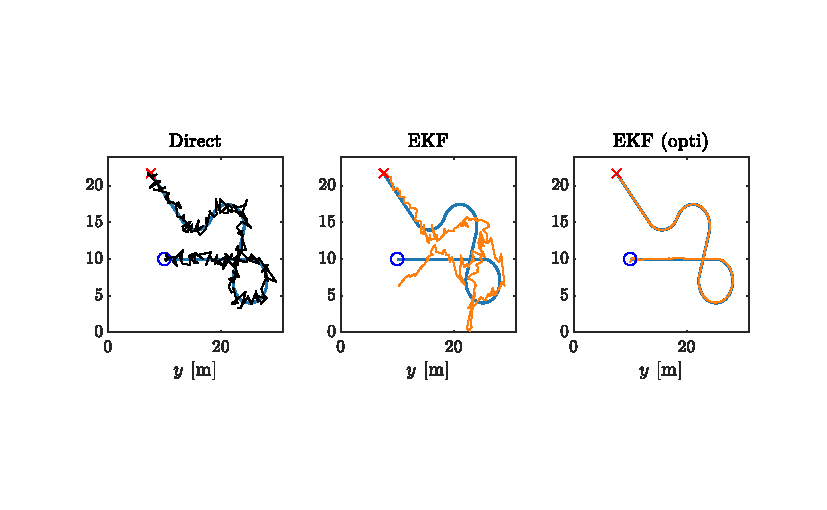
\includegraphics{figures/EKF_Le3.pdf}

The results from EKF for robot tracking with array SR implementation is 

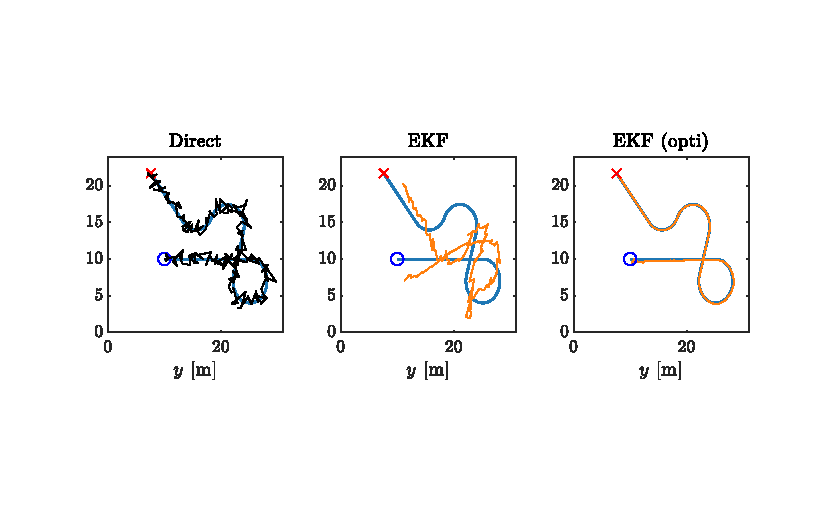
\includegraphics{figures/EKF_Le3_SR.pdf}


\fbox{\parbox{0.98\textwidth}{
    Cannot say why the SR algorithm performs much better than EKF. 
}}


% The non-linear system is 
% \begin{align*}
%     \dot X &= f(X,u)\,X, & Y &= h(X)\,X, \\
%     \text{where, } X &= \begin{pmatrix}
%         x & y & \theta
%     \end{pmatrix}^{\mathrm{T}}, & Y &= \begin{pmatrix}
%         y_1 & y_2, \\
%     \end{pmatrix}^{\mathrm{T}} \\
%     \text{and, } f(X,u) &= \begin{pmatrix}
%         V\,\cos\left(\theta\right) \\ V\,\sin\left(\theta\right) \\ u
%     \end{pmatrix} & h(X) &= \begin{pmatrix}
%         \sqrt{x^2 + y^2}, \\ \arctan{\left(\frac{y}{x}\right)},
%     \end{pmatrix}^{\mathrm{T}}
% \end{align*}


